\scanpage{131}
% archive foliation: 130
\diagram{\begin{tikzcd}X\arrow[d,"f"]\\S\end{tikzcd}}
muni d'une section $\sigma$, $f$ propre plat, $f_*\mathcal O_X=\mathcal O_S$ \uline{\unsure{universellt|universelle}}.

$G$ schéma en groupes \deleted{\unsure{plat}} fini et \deleted{\unsure{séparable}} \inserted{étale} sur $S$ [le cas important est celui où $G=S\times\Gamma$].

$F_G(T)=$ ens des classes à isom. près des fibrés principaux homogènes sur $X_T$, de groupe
\[
G_T\times_T X_T=(G\times_S X)_T\deleted{\unsure{\times X}},
\]
\uline{munis} d'une section marquée le long de $\sigma_T$, i.e. \inserted{d'un isom.} $\sigma_T^*(X')\simeq G_T$.

N.B. Tout automorphisme d'un tel \unsure{fibré} est trivial, \unsure{puisqu'on suppose que} $G$ est \deleted{\unsure{inf}} étale sur $S$. Il en serait de $=$ pour $G$ commutatif. \unsure{Cas fini}??

Le foncteur $F_G(T)$ en $T$ est-il représentable?? Si oui, le \unsure{sch.} sur $S$ qui le représente est \uline{étale} sur $S$, et \uline{quasi-fini sur $S$} [cas à fibres \uline{finies}].

Noter que le foncteur $F_G$ est \deleted{\unsure{compatible}} \unsure{ex. et à gauche} pour les morphismes fid. plats et quasi-compacts.

\margin{\figure{\begin{tikzpicture}[scale=.58,rotate=180,transform shape]
\node at (0,5.4) {\begin{minipage}{9cm}\diagram{\begin{tikzcd}[ampersand replacement=\&,column sep=small,row sep=large]
C \arrow[r,very thick] \arrow[d,no head] \& C' \arrow[r,shift left=.6ex] \arrow[r,shift right=.6ex] \arrow[d,very thick] \& C'' \arrow[r,shift left=1.2ex] \arrow[r] \arrow[r,shift right=1.2ex] \arrow[d,no head] \& C^{\prime\prime\prime} \arrow[d,no head] \\
C_{\unsure{\bullet}} \arrow[r,no head] \& C'_{\unsure{\bullet}} \arrow[r,shift left=.6ex] \arrow[r,shift right=.6ex] \& C''_{\unsure{\bullet}} \arrow[r,shift left=1.2ex] \arrow[r] \arrow[r,shift right=1.2ex] \& C^{\prime\prime\prime}_{\unsure{0}}
\end{tikzcd}}\end{minipage}};
\node at (-3.8,4.8) {\uline{\unsure{finis?}}};
\fill (-2.3,3.9) circle (.055); \fill (-.8,3.9) circle (.055);
\node at (-.7,3.45) {\uline{\unsure{fid. plat}}};
\node at (2.0,3.45) {\uline{plat}};
\draw (-1.3,2.8) .. controls (0,3.0) and (1.5,3.2) .. (2.4,2.7) .. controls (3.3,3.0) and (4,2.9) .. (4.6,3.3);
\node at (2.5,2.3) {\unsure{exacte}};
\node at (.1,-.9) {4.9.};
\node at (3.2,-.9) {\unsure{4.17.|4.13.}};
\node at (1.2,-4.3) {4.9.};
\draw (-3.2,6.6) .. controls (-1,6.4) and (1.7,6.3) .. (2.5,6.2) .. controls (2.9,5) and (2.5,0) .. (2.5,-3.8) .. controls (2.5,-4.6) and (1.4,-4.7) .. (.1,-4.6);
\draw (-1.5,6.8)--(2.0,-4.5);
\draw (-4,5.1) .. controls (-3,1) and (-1.1,-2.4) .. (-.5,-4.1);
\fill (-.5,6.9) circle (.045);
\end{tikzpicture}}}

\figure{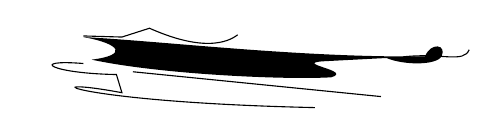
\begin{tikzpicture}[x=.7cm,y=.7cm]
\draw (0,.6)--(.7,.58)--(1.2,.74) .. controls (2.3,.25) and (2.7,.55) .. (2.8,.62);
\fill (0,.58) .. controls (.7,.45) and (.8,.25) .. (.15,.17) .. controls (1.4,-.1) and (3.7,-.2) .. (4.5,-.15) .. controls (4.9,-.03) and (3.8,.1) .. (4.35,.14) --(5.5,.2) .. controls (5.8,.07) and (6.4,.06) .. (6.5,.23) .. controls (6.6,.45) and (6.3,.49) .. (6.2,.23) .. controls (4,.2) and (1.5,.5) .. (0,.58);
\draw (0,.1) .. controls (-1,.18) and (-.6,-.08) .. (.6,-.1)--(.7,-.43) .. controls (-1,-.11) and (-.3,-.6) .. (4.2,-.7);
\draw (.9,-.05)--(5.4,-.5); \draw (5.8,.22) .. controls (6.5,.3) and (6.9,.1) .. (7,.35);
\end{tikzpicture}}

\figure{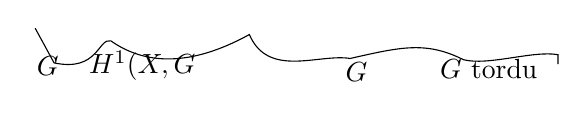
\begin{tikzpicture}[x=.8cm,y=.8cm]
\node at (0,0) {$\deleted{\unsure{G}}$};
\node at (1.5,0) {$H^1(X,G$};
\node at (4.9,-.1) {$G$};
\node at (7,-.05) {$G$ \uline{tordu}};
\draw (-.2,.6)--(.1,.05) .. controls (.8,-.1) and (.8,.45) .. (1,.4) .. controls (1.5,.05) and (2.2,-.05) .. (3.2,.5) .. controls (3.5,-.2) and (4.3,.2) .. (4.8,.12) .. controls (5.6,.3) and (6,.4) .. (6.6,.1) .. controls (7,0) and (7.7,.25) .. (8.1,.18)--(8.1,.03);
\end{tikzpicture}}
